\documentclass[../AnalysisNoteJBuxton.tex]{subfiles}
\begin{document}

\subsubsection{Results: \texorpdfstring{$\Lambda$K$^{0}_{S}$ and $\Lambda$K$^{\pm}$: 3 Residual Correlations Included in Fit}{TEXT}}
\label{ResultsLamK_3Res}


\begin{figure}[h]
  \centering
  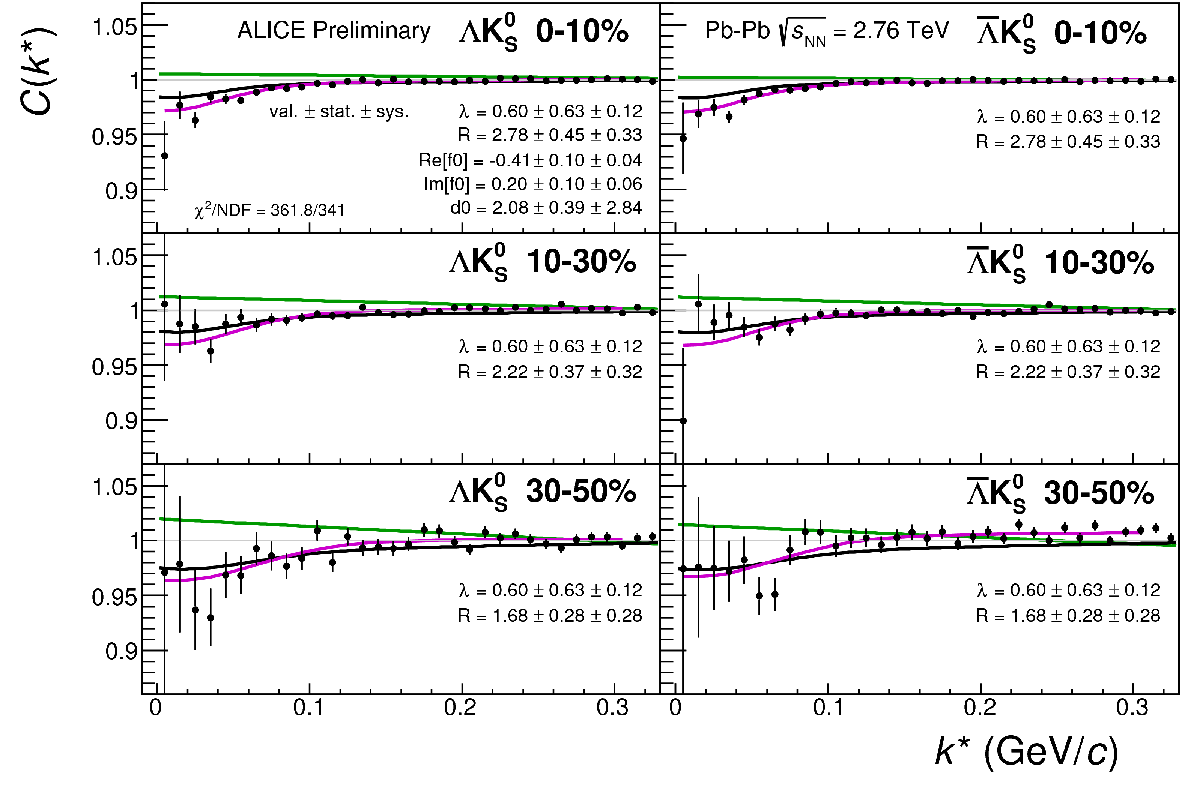
\includegraphics[width=\textwidth]{7_ResultsAndDiscussion/Figures/canKStarCfwFitsLamK0wConj_0010_1030_3050_MomResCrctn_NonFlatBgdCrctn_SingleLamParam_3Res_PrimMaxDecay4fm_UsingXiDataAndCoulombOnly.pdf}
  \caption[$\Lambda$K$^{0}_{S}$($\bar{\Lambda}$K$^{0}_{S}$) Fits with 3 Residuals]{Fits, with 3 residual correlations included, to the $\Lambda$K$^{0}_{S}$ (left) and $\bar{\Lambda}$K$^{0}_{S}$ (right) data for the centralities 0-10\% (top), 10-30\% (middle), and 30-50\% (bottom).
The lines represent the statistical errors, while the boxes represent the systematic errors.
Each has unique $\lambda$ and normalization parameters.
The radii are shared amongst like centralities; the scattering parameters ($\mathbb{R}f_{0}$, $\mathbb{I}f_{0}$, $d_{0}$) are shared amongst all.
The black solid line represents the ``raw" fit, i.e. not corrected for momentum resolution effects nor non-flat background.  
The green line shows the fit to the non-flat background.
The purple points show the fit after momentum resolution and non-flat background corrections have been applied.
The initial values of the parameters is listed, as well as the final fit values with uncertainties.
Here, $R$ was restricted to [2.,10.] and $\Lambda$ was restricted to [0.1,0.8].}
  \label{fig:LamK0wConjFits_3Res}
\end{figure}

\begin{comment}
\begin{figure}[h]
  \centering
  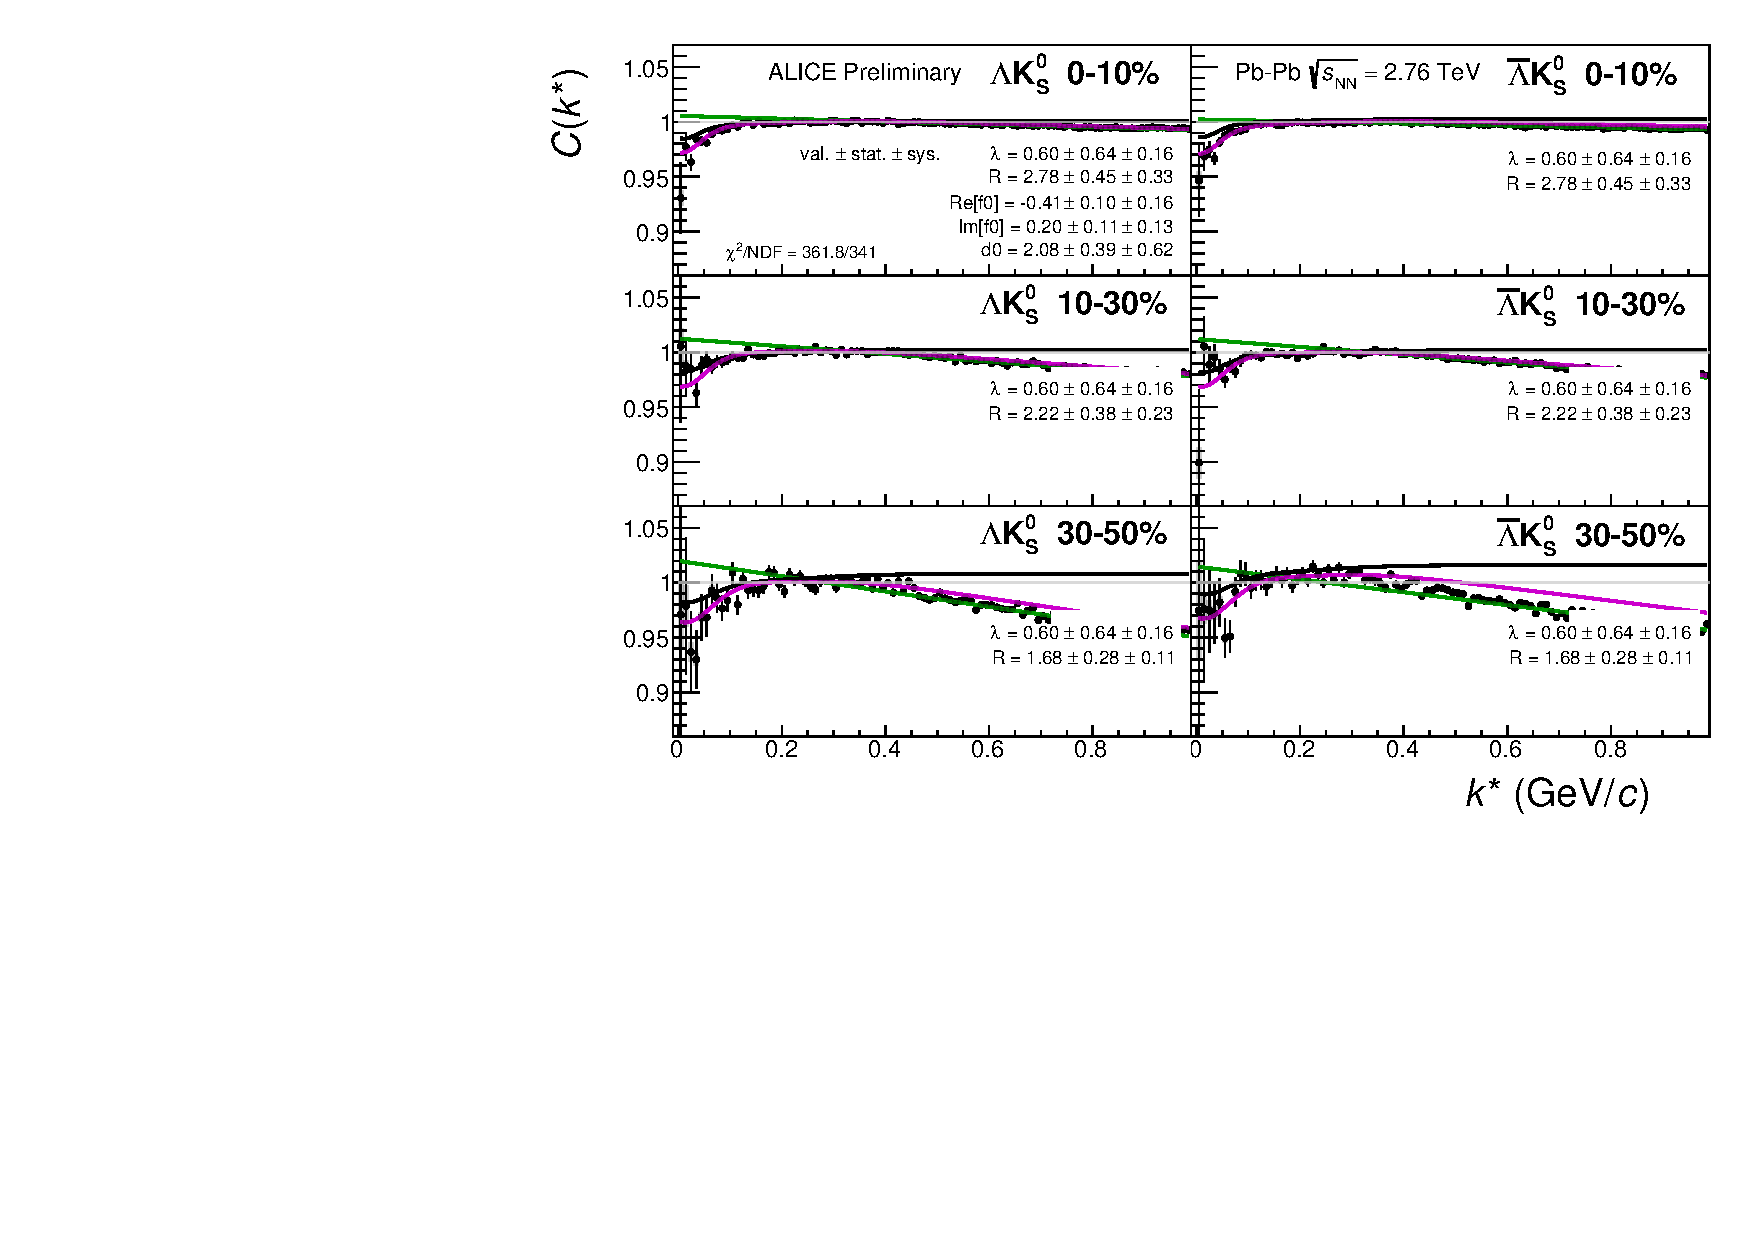
\includegraphics[width=\textwidth]{7_ResultsAndDiscussion/Figures/canKStarCfwFitsLamK0wConj_0010_1030_3050UnZoomed_MomResCrctn_NonFlatBgdCrctn_SingleLamParam_3Res_PrimMaxDecay4fm_UsingXiDataAndCoulombOnly.pdf}
  \caption[$\Lambda$K$^{0}_{S}$($\bar{\Lambda}$K$^{0}_{S}$) Fits with 3 Residuals (Wide Range)]{Same as Fig. \ref{fig:LamK0wConjFits_3Res}, but with a wider range of view.  
Fits, with 3 residual correlations included, to the $\Lambda$K$^{0}_{S}$ (left) and $\bar{\Lambda}$K$^{0}_{S}$ (right) data for the centralities 0-10\% (top), 10-30\% (middle), and 30-50\% (bottom).
The lines represent the statistical errors, while the boxes represent the systematic errors.
Each has unique $\lambda$ and normalization parameters.
The radii are shared amongst like centralities; the scattering parameters ($\mathbb{R}f_{0}$, $\mathbb{I}f_{0}$, $d_{0}$) are shared amongst all.
The black solid line represents the ``raw" fit, i.e. not corrected for momentum resolution effects nor non-flat background.  
The green line shows the fit to the non-flat background.
The purple points show the fit after momentum resolution and non-flat background corrections have been applied.
The initial values of the parameters is listed, as well as the final fit values with uncertainties.
Here, $R$ was restricted to [2.,10.] and $\Lambda$ was restricted to [0.1,0.8].}
  \label{fig:LamK0wConjFitsUnZoomed_3Res}
\end{figure}
\end{comment}



\begin{figure}[h]
  \centering
  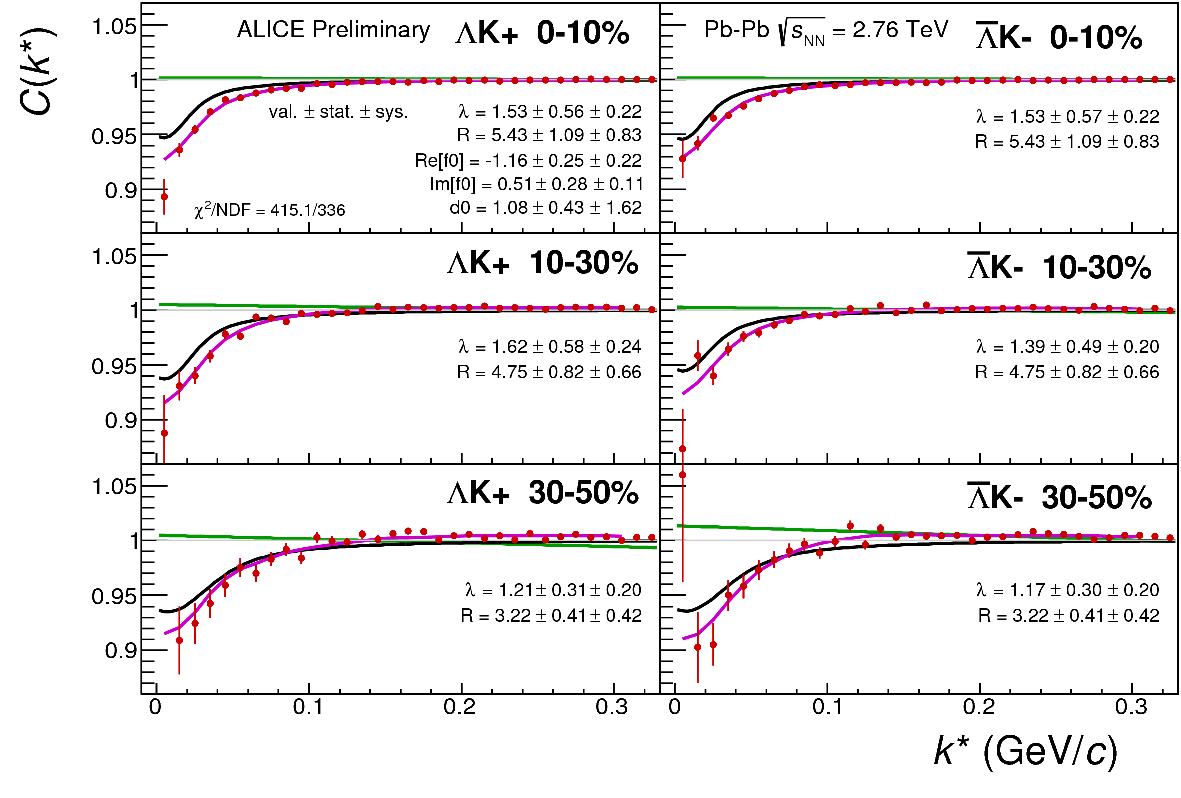
\includegraphics[width=\textwidth]{7_ResultsAndDiscussion/Figures/canKStarCfwFitsLamKchPwConj_0010_1030_3050_MomResCrctn_NonFlatBgdCrctn_3Res_PrimMaxDecay4fm_UsingXiDataAndCoulombOnly.pdf}
  \caption[$\Lambda$K$^{+}$($\bar{\Lambda}$K$^{-}$) Fits with 3 Residuals]{Fits, with 3 residual correlations included, to the $\Lambda$K$^{+}$ (left) and $\bar{\Lambda}$K$^{-}$ (right) data for the centralities 0-10\% (top), 10-30\% (middle), and 30-50\% (bottom).
The lines represent the statistical errors, while the boxes represent the systematic errors.  
Each has unique $\lambda$ and normalization parameters.
The radii are shared amongst like centralities; the scattering parameters ($\mathbb{R}f_{0}$, $\mathbb{I}f_{0}$, $d_{0}$) are shared amongst all.
The black solid line represents the ``raw" fit, i.e. not corrected for momentum resolution effects nor non-flat background.  
The green line shows the fit to the non-flat background.
The purple points show the fit after momentum resolution and non-flat background corrections have been applied.
The initial values of the parameters is listed, as well as the final fit values with uncertainties.}
  \label{fig:LamKchPwConjFits_3Res}
\end{figure}

\begin{comment}
\begin{figure}[h]
  \centering
  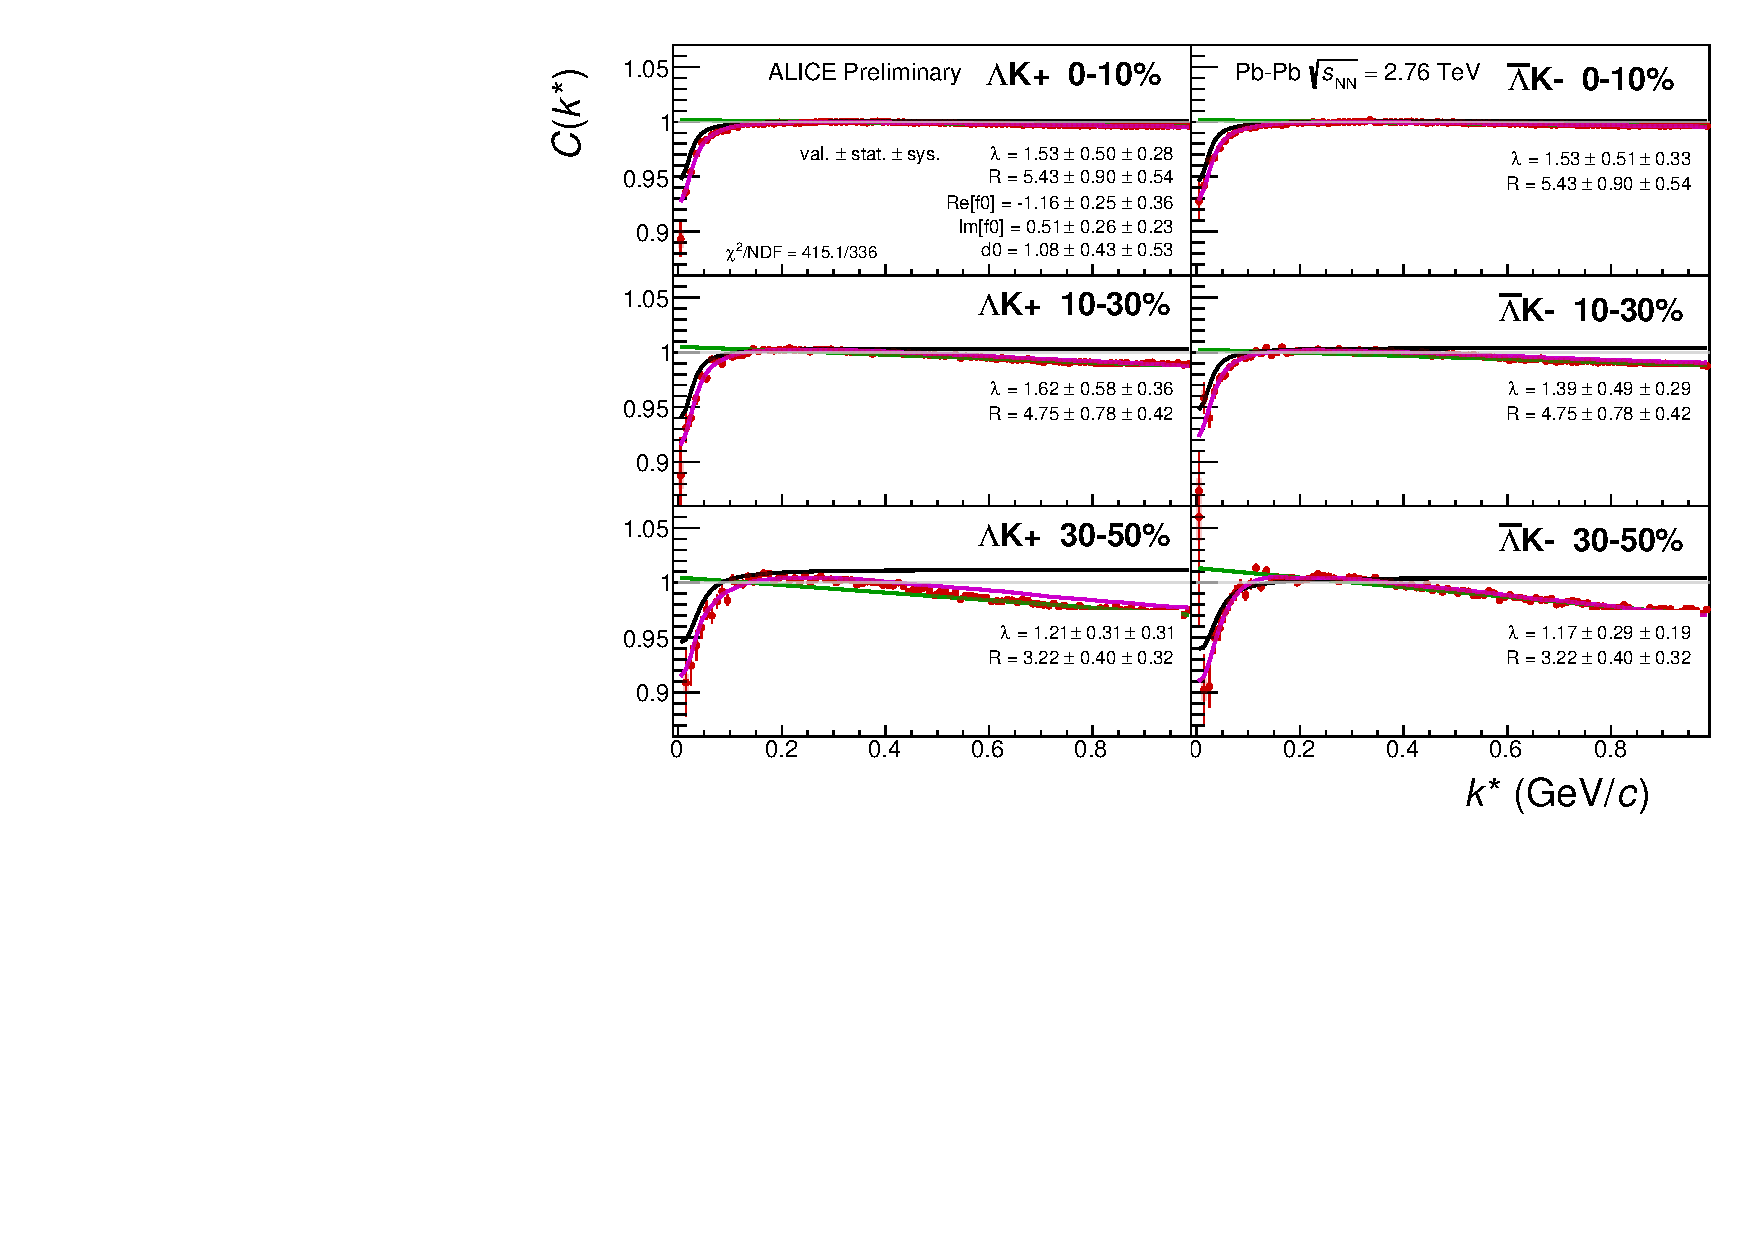
\includegraphics[width=\textwidth]{7_ResultsAndDiscussion/Figures/canKStarCfwFitsLamKchPwConj_0010_1030_3050UnZoomed_MomResCrctn_NonFlatBgdCrctn_3Res_PrimMaxDecay4fm_UsingXiDataAndCoulombOnly.pdf}
  \caption[$\Lambda$K$^{+}$($\bar{\Lambda}$K$^{-}$) Fits with 3 Residuals (Wide Range)]{Same as Fig. \ref{fig:LamKchPwConjFits_3Res}, but with a wider range of view.
Fits, with 3 residual correlations included, to the $\Lambda$K$^{+}$ (left) and $\bar{\Lambda}$K$^{-}$ (right) data for the centralities 0-10\% (top), 10-30\% (middle), and 30-50\% (bottom).
The lines represent the statistical errors, while the boxes represent the systematic errors.  
Each has unique $\lambda$ and normalization parameters.
The radii are shared amongst like centralities; the scattering parameters ($\mathbb{R}f_{0}$, $\mathbb{I}f_{0}$, $d_{0}$) are shared amongst all.
The black solid line represents the ``raw" fit, i.e. not corrected for momentum resolution effects nor non-flat background.  
The green line shows the fit to the non-flat background.
The purple points show the fit after momentum resolution and non-flat background corrections have been applied.
The initial values of the parameters is listed, as well as the final fit values with uncertainties.}
  \label{fig:LamKchPwConjFitsUnZoomed_3Res}
\end{figure}
\end{comment}



\begin{figure}[h]
  \centering
  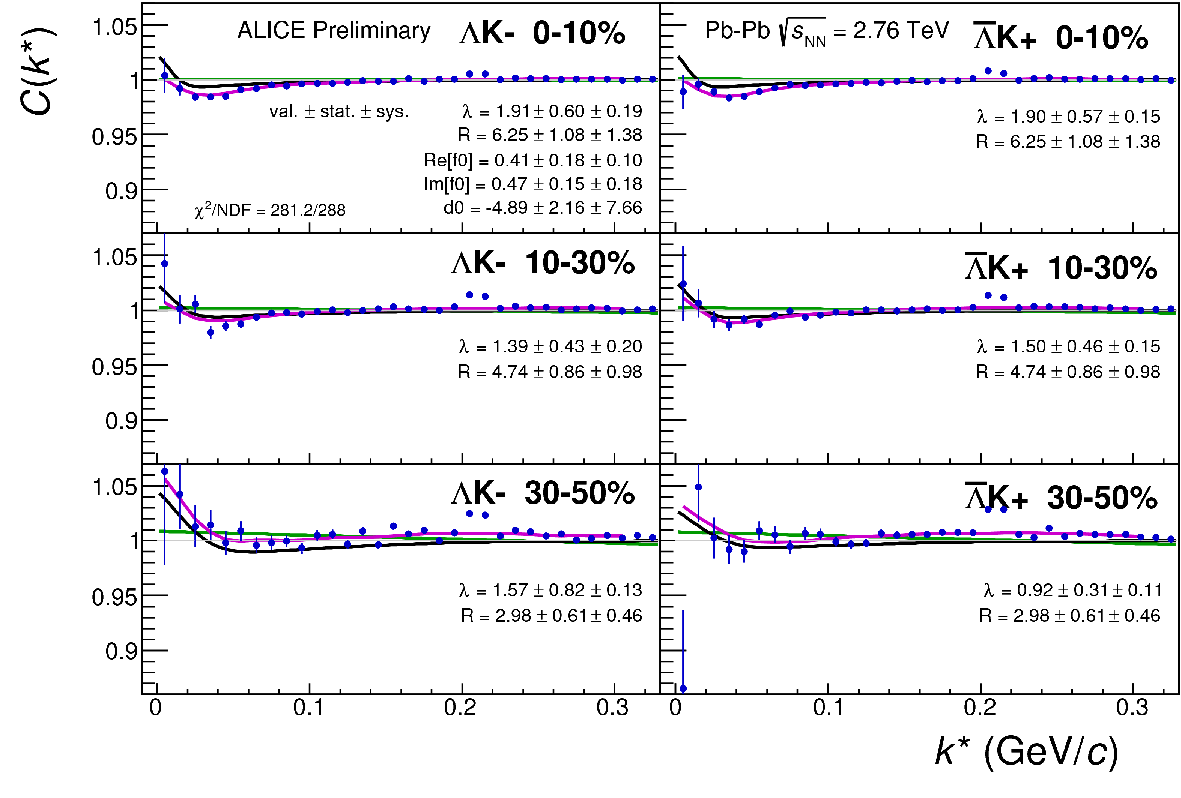
\includegraphics[width=\textwidth]{7_ResultsAndDiscussion/Figures/canKStarCfwFitsLamKchMwConj_0010_1030_3050_MomResCrctn_NonFlatBgdCrctn_3Res_PrimMaxDecay4fm_UsingXiDataAndCoulombOnly.pdf}
  \caption[$\Lambda$K$^{-}$($\bar{\Lambda}$K$^{+}$) Fits with 3 Residuals]{Fits, with 3 residual correlations included, to the $\Lambda$K$^{-}$(left) with $\bar{\Lambda}$K$^{+}$ (right) data for the centralities 0-10\% (top), 10-30\% (middle), and 30-50\% (bottom).
The lines represent the statistical errors, while the boxes represent the systematic errors.  
Each has unique $\lambda$ and normalization parameters.
The radii are shared amongst like centralities; the scattering parameters ($\mathbb{R}f_{0}$, $\mathbb{I}f_{0}$, $d_{0}$) are shared amongst all.
The black solid line represents the ``raw" fit, i.e. not corrected for momentum resolution effects nor non-flat background.  
The green line shows the fit to the non-flat background.
The purple points show the fit after momentum resolution and non-flat background corrections have been applied.
The initial values of the parameters is listed, as well as the final fit values with uncertainties.}
  \label{fig:LamKchMwConjFits_3Res}
\end{figure}

\begin{comment}
\begin{figure}[h]
  \centering
  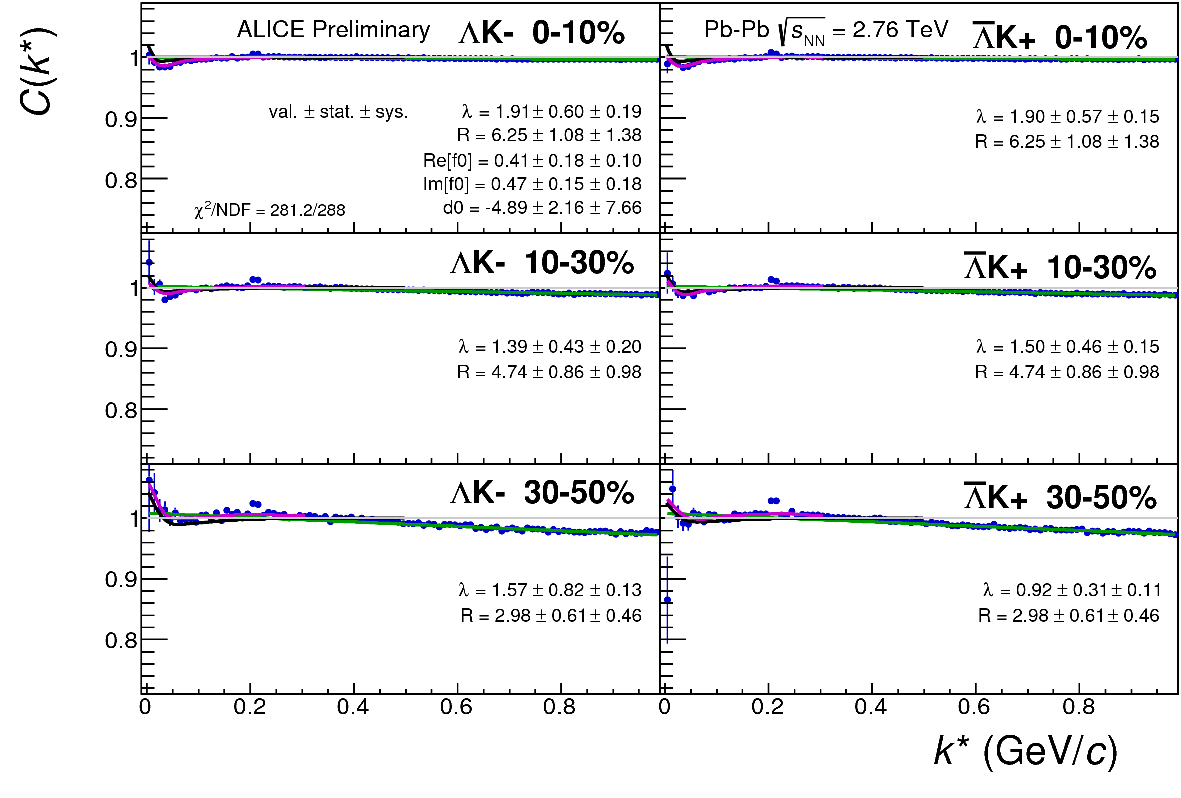
\includegraphics[width=\textwidth]{7_ResultsAndDiscussion/Figures/canKStarCfwFitsLamKchMwConj_0010_1030_3050UnZoomed_MomResCrctn_NonFlatBgdCrctn_3Res_PrimMaxDecay4fm_UsingXiDataAndCoulombOnly.pdf}
  \caption[$\Lambda$K$^{-}$($\bar{\Lambda}$K$^{+}$) Fits with 3 Residuals (Wide Range)]{Same as Fig. \ref{fig:LamKchMwConjFits_3Res}, but with a wider range of view.
Fits, with 3 residual correlations included, to the $\Lambda$K$^{-}$(left) with $\bar{\Lambda}$K$^{+}$ (right) data for the centralities 0-10\% (top), 10-30\% (middle), and 30-50\% (bottom).
The lines represent the statistical errors, while the boxes represent the systematic errors.  
Each has unique $\lambda$ and normalization parameters.
The radii are shared amongst like centralities; the scattering parameters ($\mathbb{R}f_{0}$, $\mathbb{I}f_{0}$, $d_{0}$) are shared amongst all.
The black solid line represents the ``raw" fit, i.e. not corrected for momentum resolution effects nor non-flat background.  
The green line shows the fit to the non-flat background.
The purple points show the fit after momentum resolution and non-flat background corrections have been applied.
The initial values of the parameters is listed, as well as the final fit values with uncertainties.}
  \label{fig:LamKchMwConjFitsUnZoomed_3Res}
\end{figure}
\end{comment}

\begin{comment}
\pagestyle{empty}
\begin{landscape}

\begin{table}[htbp]
 \centering
 \resizebox{\paperwidth}{!}{
 \begin{tabular}{|c|c|c|c|c|c|c|}
  \multicolumn{7}{c}{Fit Results $\Lambda$($\bar{\Lambda}$)K$^{0}_{S}$} \\
  \hline
  \multirow{3}{*}{Pair Type} & \multirow{3}{*}{Centrality} & \multicolumn{5}{c|}{Fit Parameters} \\
  \cline{3-7}
   & & $\lambda$ & $R$ & $\mathbb{R}f_{0}$ & $\mathbb{I}f_{0}$ & $d_{0}$ \\
  \hline  
  \multirow{3}{*}{$\Lambda$K$^{0}_{S}$}  
   &  0-10\% & \multirow{6}{*}{0.400 $\pm$ 0.187 (stat.) $\pm$ 0.116 (sys.)}  %Lambda
             & 3.024 $\pm$ 0.541 (stat.) $\pm$ 0.329 (sys.)  %Radius
             & \multirow{6}{*}{-0.157 $\pm$ 0.031 (stat.) $\pm$ 0.043 (sys.)}  %Ref0
             & \multirow{6}{*}{0.176 $\pm$ 0.077 (stat.) $\pm$ 0.059 (sys.)}  %Imf0
             & \multirow{6}{*}{3.566 $\pm$ 0.947 (stat.) $\pm$ 2.836 (sys.)} \\ %d0
             
   & 10-30\% & 
             & 2.270 $\pm$ 0.413 (stat.) $\pm$ 0.324 (sys.)  %Radius
             & & & \\
             
   & 30-50\% & 
             & 1.669 $\pm$ 0.307 (stat.) $\pm$ 0.280 (sys.)  %Radius
             & & & \\
  \cline{1-2}
  \cline{4-4}
  \multirow{3}{*}{$\bar{\Lambda}$K$^{0}_{S}$}  
   &  0-10\% & 
             & 3.024 $\pm$ 0.541 (stat.) $\pm$ 0.329 (sys.)  %Radius
             & & & \\
             
   & 10-30\% & 
             & 2.270 $\pm$ 0.413 (stat.) $\pm$ 0.324 (sys.)  %Radius
             & & & \\
             
   & 30-50\% & 
             & 1.669 $\pm$ 0.307 (stat.) $\pm$ 0.280 (sys.)  %Radius
             & & & \\
  \hline
 \end{tabular}}
 \caption{Fit Results $\Lambda$($\bar{\Lambda}$)K$^{0}_{S}$, with 3 residual correlations included. 
 Each pair is fit simultaneously with its conjugate (ie. $\Lambda$K$^{0}_{S}$ with $\bar{\Lambda}$K$^{0}_{S}$) across all centralities (0-10\%, 10-30\%, 30-50\%), for a total of 6 simultaneous analyses in the fit.
 Each analysis has a unique $\lambda$ and normalization parameter.
 The radii are shared between analyses of like centrality, as these should have similar source sizes.
 The scattering parameters ($\mathbb{R}f_{0}$, $\mathbb{I}f_{0}$, $d_{0}$) are shared amongst all.
 The fit is done on the data with only statistical error bars.
 The errors marked as ``stat." are those returned by MINUIT.
 The errors marked as ``sys." are those which result from my systematic analysis (as outlined in Section \ref{SystematicErrors}).}
 \label{tab:FitResultsLamK0_3Res}
\end{table}



%\end{landscape}
%\pagestyle{plain}

%\pagestyle{empty}
%\begin{landscape}

\begin{table}[htbp]
 \centering
 \resizebox{\paperwidth}{!}{
 \begin{tabular}{|c|c|c|c|c|c|c|}
  \multicolumn{7}{c}{Fit Results $\Lambda$($\bar{\Lambda}$)K$^{\pm}$} \\
  \hline
  \multirow{3}{*}{Pair Type} & \multirow{3}{*}{Centrality} & \multicolumn{5}{c|}{Fit Parameters} \\
  \cline{3-7}
   & & $\lambda$ & $R$ & $\mathbb{R}f_{0}$ & $\mathbb{I}f_{0}$ & $d_{0}$ \\
  \hline  
  \multirow{3}{*}{$\Lambda$K$^{+}$}  
   &  0-10\% & 0.379 $\pm$ 0.085 (stat.) $\pm$ 0.220 (sys.)  %Lambda
             & 4.045 $\pm$ 0.381 (stat.) $\pm$ 0.830 (sys.)  %Radius
             & \multirow{6}{*}{-0.687 $\pm$ 0.160 (stat.) $\pm$ 0.223 (sys.)}  %Ref0
             & \multirow{6}{*}{0.391 $\pm$ 0.143 (stat.) $\pm$ 0.111 (sys.)}  %Imf0
             & \multirow{6}{*}{0.639 $\pm$ 0.534 (stat.) $\pm$ 1.621 (sys.)} \\ %d0
             
   & 10-30\% & 0.485 $\pm$ 0.129 (stat.) $\pm$ 0.241 (sys.)  %Lambda
             & 3.923 $\pm$ 0.454 (stat.) $\pm$ 0.663 (sys.)  %Radius
             & & & \\
             
   & 30-50\% & 0.639 $\pm$ 0.195 (stat.) $\pm$ 0.204 (sys.)  %Lambda
             & 3.717 $\pm$ 0.554 (stat.) $\pm$ 0.420 (sys.)  %Radius
             & & & \\
  \cline{1-4}  
  \multirow{3}{*}{$\bar{\Lambda}$K$^{-}$}  
   &  0-10\% & 0.371 $\pm$ 0.083 (stat.) $\pm$ 0.217 (sys.)  %Lambda
             & 4.045 $\pm$ 0.381 (stat.) $\pm$ 0.830 (sys.)  %Radius
             & & & \\
             
   & 10-30\% & 0.411 $\pm$ 0.111 (stat.) $\pm$ 0.201 (sys.)  %Lambda
             & 3.923 $\pm$ 0.454 (stat.) $\pm$ 0.663 (sys.)  %Radius
             & & & \\
             
   & 30-50\% & 0.616 $\pm$ 0.192 (stat.) $\pm$ 0.203 (sys.)  %Lambda
             & 3.717 $\pm$ 0.554 (stat.) $\pm$ 0.420 (sys.)  %Radius
             & & & \\
  \hline
  \hline  
  \multirow{3}{*}{$\Lambda$K$^{-}$}  
   &  0-10\% & 1.91 $\pm$ 0.60 (stat.) $\pm$ 0.19 (sys.)  %Lambda
             & 6.25 $\pm$ 1.08 (stat.) $\pm$ 1.38 (sys.)  %Radius
             & \multirow{6}{*}{0.41 $\pm$ 0.18 (stat.) $\pm$ 0.10 (sys.)}  %Ref0
             & \multirow{6}{*}{0.47 $\pm$ 0.15 (stat.) $\pm$ 0.18 (sys.)}  %Imf0
             & \multirow{6}{*}{-4.89 $\pm$ 2.16 (stat.) $\pm$ 7.66 (sys.)} \\ %d0
             
   & 10-30\% & 1.39 $\pm$ 0.43 (stat.) $\pm$ 0.20 (sys.)  %Lambda
             & 4.74 $\pm$ 0.86 (stat.) $\pm$ 0.98 (sys.)  %Radius
             & & & \\
             
   & 30-50\% & 1.57 $\pm$ 0.82 (stat.) $\pm$ 0.13 (sys.)  %Lambda
             & 2.98 $\pm$ 0.61 (stat.) $\pm$ 0.46 (sys.)  %Radius
             & & & \\
  \cline{1-4}  
  \multirow{3}{*}{$\bar{\Lambda}$K$^{+}$}  
   &  0-10\% & 1.90 $\pm$ 0.57 (stat.) $\pm$ 0.15 (sys.)  %Lambda
             & 6.25 $\pm$ 1.08 (stat.) $\pm$ 1.38 (sys.)  %Radius
             & & & \\
             
   & 10-30\% & 1.50 $\pm$ 0.46 (stat.) $\pm$ 0.15 (sys.)  %Lambda
             & 4.74 $\pm$ 0.86 (stat.) $\pm$ 0.98 (sys.)  %Radius
             & & & \\
             
   & 30-50\% & 0.92 $\pm$ 0.31 (stat.) $\pm$ 0.11 (sys.)  %Lambda
             & 2.98 $\pm$ 0.61 (stat.) $\pm$ 0.46 (sys.)  %Radius
             & & & \\
  \hline
 \end{tabular}}
 \caption{Fit Results $\Lambda$($\bar{\Lambda}$)K$^{\pm}$, with 3 residual correlations included.
 Each pair is fit simultaneously with its conjugate (ie. $\Lambda$K$^{+}$ with $\bar{\Lambda}$K$^{-}$ and $\Lambda$K$^{-}$ with $\bar{\Lambda}$K$^{+}$) across all centralities (0-10\%, 10-30\%, 30-50\%), for a total of 6 simultaneous analyses in the fit.
 Each analysis has a unique $\lambda$ and normalization parameter.
 The radii are shared between analyses of like centrality, as these should have similar source sizes.
 The scattering parameters ($\mathbb{R}f_{0}$, $\mathbb{I}f_{0}$, $d_{0}$) are shared amongst all.
 The fit is done on the data with only statistical error bars.
 The errors marked as ``stat." are those returned by MINUIT.
 The errors marked as ``sys." are those which result from my systematic analysis (as outlined in Section \ref{SystematicErrors}).}
 \label{tab:FitResultsLamKch_3Res}
\end{table}


%%%%%%%%%%%%%%%%%%%%%%%%%%%%%%%%%%%%%%%%%%%%%%%%%%%%%%%%%%%%%%%%%%%%%%%%%%%%%%%%%%%%%%%%%%%%%
%%%%%%%%%%%%%%%%%% QM 17 Stuff %%%%%%%%%%%%%%%%%%%%%%%%%%%%%%%%%%%%%%%%%%%%%%%%%%%%%%%%%%%%%%

\clearpage
\begin{table}[htbp]
 \centering
 \resizebox{\paperwidth}{!}{
 \begin{tabular}{|c|c|c|c|c|}
  \multicolumn{2}{c}{} & \multicolumn{3}{c}{\textbf{\large Fit Parameters} (\large \textbf{value $\pm$ statistical error $\pm$ systematic error)}} \\
  \hline
  \textbf{\large Pair Type} & \textbf{\large Centrality} & \multicolumn{3}{c|}{\textbf{\large R}} \\
  \cline{1-5}
  \multirow{5}{*}{\large \textbf{$\Lambda$K$^{+}$ \& $\bar{\Lambda}$K$^{-}$}}
  &  \textbf{0-10\%} & \multicolumn{3}{c|}{\textbf{4.04 $\pm$ 0.38 $\pm$ 0.83}} \\  %Radius
  & \textbf{10-30\%} & \multicolumn{3}{c|}{\textbf{3.92 $\pm$ 0.45 $\pm$ 0.66}} \\  %Radius
  & \textbf{30-50\%} & \multicolumn{3}{c|}{\textbf{3.72 $\pm$ 0.55 $\pm$ 0.42}} \\  %Radius
  \cline{2-5}
  & & \large $\mathbf{\Re f_{0}}$ & \large $\mathbf{\Im f_{0}}$ & \large $\mathbf{d_{0}}$ \\
  \cline{3-5}  
  & & \textbf{-0.69 $\pm$ 0.16 $\pm$ 0.22} & \textbf{0.39 $\pm$ 0.14 $\pm$ 0.11} & \textbf{0.64 $\pm$ 0.53 $\pm$ 1.62} \\
  
  \hline
  \hline
  
  \multirow{5}{*}{\large \textbf{$\Lambda$K$^{-}$ \& $\bar{\Lambda}$K$^{+}$}} 
  &  \textbf{0-10\%} & \multicolumn{3}{c|}{\textbf{4.79 $\pm$ 0.79 $\pm$ 1.38}} \\  %Radius
  & \textbf{10-30\%} & \multicolumn{3}{c|}{\textbf{4.00 $\pm$ 0.72 $\pm$ 0.98}} \\  %Radius
  & \textbf{30-50\%} & \multicolumn{3}{c|}{\textbf{2.11 $\pm$ 0.52 $\pm$ 0.46}} \\  %Radius
  \cline{2-5}
  & & \large $\mathbf{\Re f_{0}}$ & \large $\mathbf{\Im f_{0}}$ & \large $\mathbf{d_{0}}$ \\
  \cline{3-5}     
  & & \textbf{0.18 $\pm$ 0.13 $\pm$ 0.10} & \textbf{0.45 $\pm$ 0.18 $\pm$ 0.18} & \textbf{-5.29 $\pm$ 2.94 $\pm$ 7.66} \\
   
  \hline
  \hline  
  
  \multirow{5}{*}{\large \textbf{$\Lambda$K$^{0}_{S}$ \& $\bar{\Lambda}$K$^{0}_{S}$}}  
   &  \textbf{0-10\%} & \multicolumn{3}{c|}{\textbf{3.02 $\pm$ 0.54 $\pm$ 0.33}} \\  %Radius
   & \textbf{10-30\%} & \multicolumn{3}{c|}{\textbf{2.27 $\pm$ 0.41 $\pm$ 0.32}} \\  %Radius
   & \textbf{30-50\%} & \multicolumn{3}{c|}{\textbf{1.67 $\pm$ 0.30 $\pm$ 0.28}} \\  %Radius
   \cline{2-5}   
   & & \large $\mathbf{\Re f_{0}}$ & \large $\mathbf{\Im f_{0}}$ & \large $\mathbf{d_{0}}$ \\
   \cline{3-5} 
   & & \textbf{-0.16 $\pm$ 0.03 $\pm$ 0.04} & \textbf{0.18 $\pm$ 0.08 $\pm$ 0.06} & \textbf{3.57 $\pm$ 0.95 $\pm$ 2.84} \\
  \hline
 \end{tabular}}
 \caption{Fit Results $\Lambda$($\bar{\Lambda}$)K$^{\pm}$ and $\Lambda$($\bar{\Lambda}$)K$^{0}_{\mathrm{S}}$, with 3 residual correlations included ($\lambda$ parameters not shown).  This table is a condensed version of Tables \ref{tab:FitResultsLamK0_3Res} and \ref{tab:FitResultsLamKch_3Res}} 
 \label{tab:FitResultsLamKCondensed_3Res}
\end{table}

\end{landscape}
\pagestyle{plain}
\end{comment}

\begin{figure}[h]
  \centering
  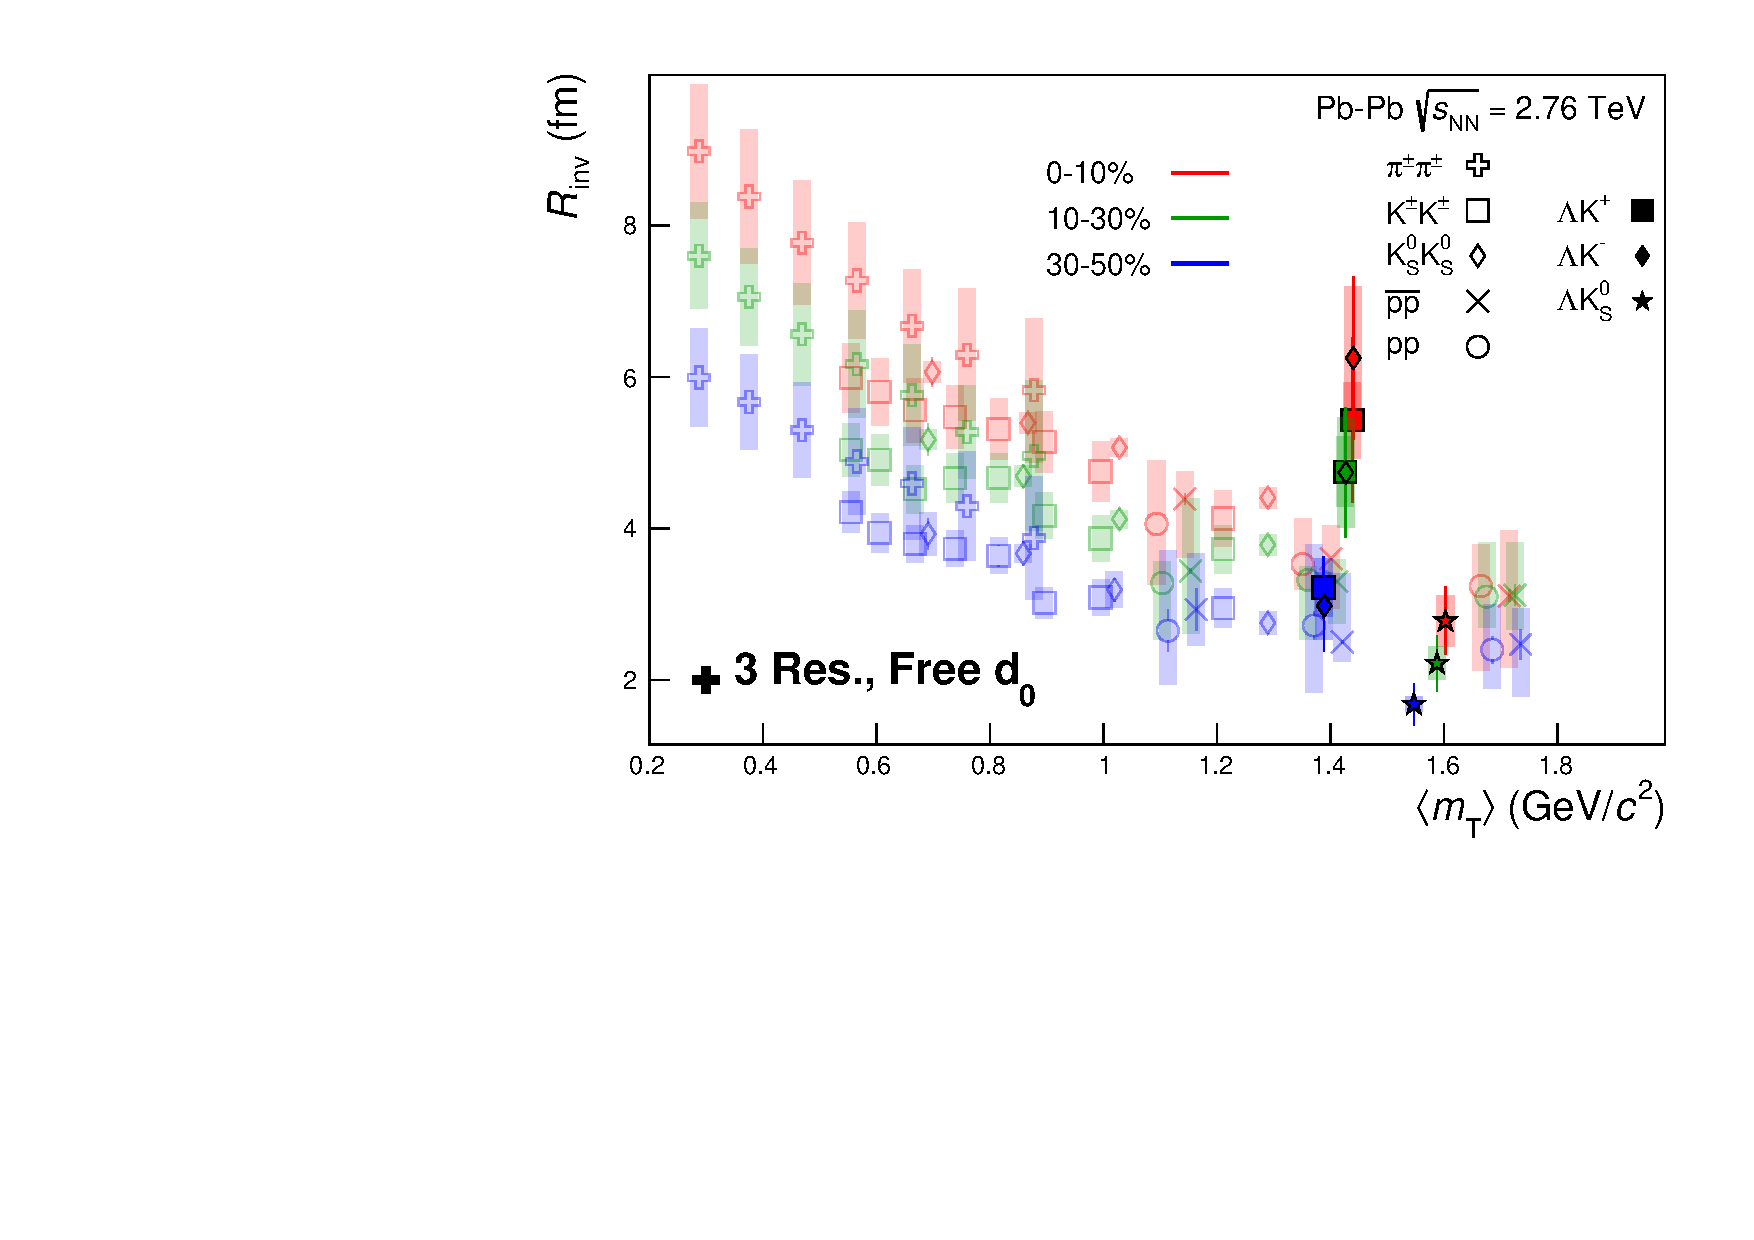
\includegraphics[width=\textwidth]{7_ResultsAndDiscussion/Figures/mTscaling_MinvCalc_OutlinedPoints_OthersTransparent_3Res_FreeD0.pdf}
  \caption[$m_{\mathrm{T}}$ Scaling of Radii: 3 Residuals in Fit]{3 residual correlations in $\Lambda$K fits.  Extracted fit $R_{\mathrm{inv}}$ parameters as a function of pair transverse mass ($m_{\mathrm{T}}$) for various pair systems over several centralities. The ALICE published data \cite{Adam:2015vja} is shown with transparent, open symbols.  The new $\Lambda$K results are shown with opaque, filled symbols.  In the left, the $\Lambda$K$^{+}$ (with it's conjugate pair) results are shown separately from the $\Lambda$K$^{-}$ (with it's conjugate pair) results.  In the right, all $\Lambda$K$^{\pm}$ results are averaged.}
  \label{fig:mTScalingOfRadii_3Res}
\end{figure}

\clearpage

\end{document}